\chapter{Triangle Quality Metrics}

All the metrics in this section are defined on a triangular element
as illustrated in Figure~\ref{f:tri}.

\begin{figure}[bhp]
  \centering
  \includegraphics[width=2in]{tri}
  \caption{Numbering of vertices and edges on a triangular element.%
                                                                  \label{f:tri}}
\end{figure}

Note that unlike all the other elements that follow,
we name edge vectors of the triangle by the vertex opposite the edge so that
\begin{equation*}
\begin{array}{lcl}
  \vec L_0 &=& \vec P_2 - \vec P_1\\
  \vec L_1 &=& \vec P_0 - \vec P_2\\
  \vec L_2 &=& \vec P_1 - \vec P_0.
\end{array}
\end{equation*}

The triangle edge lengths are denoted as follows:
\[
L_0 = \normvec{L_0}\quad
L_1 = \normvec{L_1}\quad
L_2 = \normvec{L_2}
\]
and the largest and smallest edge lengths are, respectively,
\[
L_{\min} = \min\left(L_0, L_1, L_2\right)
  \rule{2em}{0pt}
L_{\max} = \max\left(L_0, L_1, L_2\right)
\]

The area of a triangle is one half the magnitude of the cross product of any pair of adjacent edge vectors:
\begin{equation*}
  A
    = \frac{1}{2}\normvec{L_0\times\vec L_1}
    = \frac{1}{2}\normvec{L_1\times\vec L_2}
    = \frac{1}{2}\normvec{L_2\times\vec L_0}
\end{equation*}

In addition, we will let $r$ be the inradius
\begin{equation*}
\label{eq:Arp}
  r = \frac{2A}{\normvec{L_0} + \normvec{L_1} + \normvec{L_2}}
\end{equation*}
and $R$ the circumradius
\[
  R = \frac{\normvec{L_0} \normvec{L_1} \normvec{L_2}}%
           {2 r \left(\normvec{L_0} + \normvec{L_1} + \normvec{L_2}\right)}
\]
of the triangle.
These are respectively the radii of the inscribed and circumscribed circles of this triangle.

We will frequently use $n$ to represent some arbitrary edge $L_n$ or vertex $P_n$ of the triangle.
When referring to the next counterclockwise entry $n+1$ (or clockwise entry $n-1$),
we take the result modulo $3$ so that, for example, if $n = 1$, $n+1 = 2$ and $n+2 = 0$.

% -------------------Metric Table-------------------
\newcommand{\trimetrictable}[8]{%
  \begin{center}
  \begin{tabular}{ll}
    \multicolumn{2}{r}{\textbf{\sffamily\Large triangle #1}}\\\hline
    Dimension:                           & #2\\ 
    Acceptable Range:                    & #3\\ 
    Normal Range:                        & #4\\ 
    Full Range:                          & #5\\ 
    $q$ for equilateral unit triangle:   & #6\\
    Reference:                           & #7\\
    \verd\ function:       & \texttt{#8}\\ \hline
  \end{tabular} 
  \end{center}
}

\newpage %---------------------------Area-----------------------------
\section{Area\label{s:tri-area}}

This metric is simply the area as defined above
\[
  q = A.
\]

Note that since $A$ is non-negative, the current version of \verd\ cannot detect inverted triangles.
What are you doing with inverted triangles, anyway? There's only 3 vertices to keep track of!

\trimetrictable{area}%
{$L^2$}%                                              Dimension
{$[0,DBL\_MAX]$}%                                     Acceptable range
{$[0,DBL\_MAX]$}%                                     Normal range
{$[0,DBL\_MAX]$}%                                     Full range
{$\frac{\sqrt{3}}{4}$}%                               Unit equilateral triangle value
{--}%                                                 Reference(s)
{v\_tri\_area}%                            Verdict function name
  
  
  
  
  
  

\newpage %---------------------------Aspect Ratio-----------------------------
\section{Aspect Ratio\label{s:tri-aspect-ratio}}

The aspect ratio of a triangle is: 
\[
q = \frac{L_{\max}}{2\sqrt{3}r}.
\]
Using~\eqref{eq:Arp}, one can thus write it alternatively as
\begin{equation*}
\label{eq:triangle_aspect_ratio}
q = \frac{L_{\max}(L_0 + L_1 + L_2)}{4\sqrt{3}A}.
\end{equation*}

Note that in earlier versions of \verd{}, triangle aspect ratio
was used to call out what is now called the triangle aspect.

\trimetrictable{aspect ratio}%
{$1$}%                                                Dimension
{$[1,1.3]$}%                                          Acceptable range
{$[1,DBL\_MAX]$}%                                     Normal range
{$[1,DBL\_MAX]$}%                                     Full range
{$1$}%                                                Unit equilateral triangle value
{\cite{pebay:03}}%                                    Reference(s)                   
{v\_tri\_aspect\_ratio}%                            Verdict function name


\newpage %---------------------------Aspect Frobenius-----------------------------
\section{Aspect Frobenius\label{s:tri-aspect-Frobenius}}

The aspect Frobenius is the sum of the edge lengths squared divided by the area
and normalized so that a unit equilateral triangle has a value of $1$.
\[
  q = \frac{{\normvec{{L_0}}}^{2} +
            {\normvec{{L_1}}}^{2} + 
            {\normvec{{L_2}}}^{2}}{4A\sqrt{3}}
\]

Note that in earlier versions of \verd{}, this metric was
called the triangle aspect ratio.

\trimetrictable{aspect Frobenius}%
{$1$}%                                                Dimension
{$[1,1.3]$}%                                          Acceptable range
{$[1,DBL\_MAX]$}%                                     Normal range
{$[1,DBL\_MAX]$}%                                     Full range
{$1$}%                                                Unit equilateral triangle value
{\cite{pebay:03}}%                                    Reference(s)                   
{v\_tri\_aspect\_frobenius}%                            Verdict function name


\newpage %---------------------------Condition Number-----------------------------
\section{Condition\label{s:tri-condition}}

The condition number of the weighted Jacobian matrix is
\[
  q = \frac{
    \left(\vec L_2\cdot\vec L_2 + \vec L_1\cdot\vec L_1 + \vec L_1\cdot\vec L_2 \right)}%
    {2A\sqrt{3}}.
\]

Note that when $A = 0$, we set $q = DBL\_MAX$.
In theory the condition number is invariant to which node it is computed at,
but floating point truncation error can contribute to differences between
values computed for each node.
\verd\ always uses the first vertex.

\trimetrictable{condition}%
{$1$}%                                                Dimension
{$[1,1.3]$}%                                          Acceptable range
{$[1,DBL\_MAX]$}%                                     Normal range
{$[1,DBL\_MAX]$}%                                     Full range
{$1$}%                                                Unit equilateral triangle value
{\cite{knu:00,knu:03}}%                               Reference(s)                   
{v\_tri\_condition}%                            Verdict function name


\newpage %---------------------------Distortion-----------------------------
\section{Distortion\label{s:tri-distortion}}

Let $A$ be the area as defined in \S\ref{s:tri-area}
and $A_m = \sqrt{3}$ be the area of a ``master'' triangle with vertices
\[
\begin{array}{lcrcrcrl}
  \vec P_0 &= (&-1&,& -\frac{ \sqrt{3}}{3}&,& 0&)\\
  \vec P_1 &= (& 1&,& -\frac{ \sqrt{3}}{3}&,& 0&)\\
  \vec P_2 &= (& 0&,&  \frac{2\sqrt{3}}{3}&,& 0&).
\end{array}
\]
Now define $|J|$ as the minimum value of the
determinant of the Jacobian evaluated at all Gauss points of the element.
The distortion is then
\[
q = \frac{|J| A_m}{A} = \frac{|J|\sqrt{3}}{A}.
\]
Distortion is a measure of how well-behaved the mapping from
parameter space to world coordinates is.

Note that this metric is currently unsupported.

\trimetrictable{distortion}%
{$1$}%                                                Dimension
{$[0.5,1]$}%                                          Acceptable range
{$[0,1]$}%                                            Normal range
{$[-DBL\_MAX,DBL\_MAX]$}%                             Full range
{$1$}%                                                Unit equilateral triangle value
{Adapted from \cite{ideas:xx}}%                       Reference(s)                   
{v\_tri\_distortion}%                            Verdict function name


\newpage %---------------------------Edge Ratio-----------------------------
\section{Edge Ratio}

The edge ratio of a triangle is: 
\[
\frac{L_{\max}}{L_{\min}}.
\]

\trimetrictable{edge ratio}%
{$1$}%                                      Dimension
{$[1,1.3]$}%                                Acceptable range
{$[1,DBL\_MAX]$}%                           Normal range
{$[1,DBL\_MAX]$}%                           Full range
{$1$}%                                      Square
{\cite{pebay:03}}%                          Citation
{v\_tri\_edge\_ratio}%                            Verdict function name


\newpage %---------------------------Maximum Angle-----------------------------
\section{Maximum Angle\label{s:tri-max-angle}}

The maximum included angle of the triangle is
\[
  q =
    \max_{n\in\{0,1,2\}}\left\{\arccos{\left(
      \frac{\vec L_n\cdot\vec L_{n+1}}{\normvec{ L_n}\normvec{ L_{n+1}}}
    \right)}\left(\frac{180\dgr}{\pi}\right)\right\}
\]
measured in degrees.

Note that if any edge vector has zero length, \verd\ will return $q = 0\dgr$.

\trimetrictable{maximum included angle}%
{$A^1$}%                                              Dimension
{$[60\dgr,90\dgr]$}%                                  Acceptable range
{$[60\dgr,180\dgr]$}%                                 Normal range
{$[0\dgr,180\dgr]$}%                                  Full range
{$60\dgr$}%                                           Unit equilateral triangle value
{--}%                                                 Reference(s)                   
{v\_tri\_maximum\_angle}%                             Verdict function name


\newpage %---------------------------Minimum Angle-----------------------------
\section{Minimum Angle\label{s:tri-min-angle}}

The minimum included angle of the triangle is
\[
  q =
    \min_{n\in\{0,1,2\}}\left\{\arccos{\left(
      \frac{\vec L_n\cdot\vec L_{n+1}}{\normvec{ L_n}\normvec{ L_{n+1}}}
    \right)}\left(\frac{180\dgr}{\pi}\right)\right\}
\]
measured in degrees.

Note that if any edge vector has zero length, \verd\ will return $q = 360\dgr$.

\trimetrictable{minimum included angle}%
{$A^1$}%                                              Dimension
{$[30\dgr,60\dgr]$}%                                  Acceptable range
{$[0\dgr,60\dgr]$}%                                   Normal range
{$[0\dgr,360\dgr]$}%                                  Full range
{$60\dgr$}%                                           Unit equilateral triangle value
{\cite{pebay:03}}%                                    Reference(s)                   
{v\_tri\_minimum\_angle}%                             Verdict function name


\newpage %---------------------------Scaled Jacobian-----------------------------
\section{Scaled Jacobian\label{s:tri-scaled-jacobian}}

First, let $L_{\max}$ be the product of the lengths of the 2 longest edges:
\[
  L_{\max} = \max\left\{
    \normvec{ L_0} \normvec{ L_1},
    \normvec{ L_0} \normvec{ L_2},
    \normvec{ L_1} \normvec{ L_2}
  \right\}
\]
Let $J^{\prime}$ be the Jacobian of the triangle.
If the triangle surface normal $\hat n$ is evaluated at the center of the triangle
and $\hat n\cdot\left(\vec L_2\times\vec L_1\right) < 0$, then take $J = -J^{\prime}$.
Otherwise take $J = J^{\prime}$.
The scaled Jacobian is then
\[
  q = \frac{2\sqrt{3}}{3} \frac{J}{L_{\max}}
\]
which is normalized so that a unit equilateral triangle has value $1$.

Note that if $L_{\max} \leq DBL\_MIN$, we set $q = 0$.

\trimetrictable{scaled Jacobian}%
{$1$}%                                                Dimension
{$[0.5,\frac{2\sqrt{3}}{3}]$}%                        Acceptable range
{$[-\frac{2\sqrt{3}}{3},\frac{2\sqrt{3}}{3}]$}%       Normal range
{$[-DBL\_MAX,DBL\_MAX]$}%                             Full range
{$1$}%                                                Unit equilateral triangle value
{\cite{knu:00}}%                                      Reference(s)                   
{v\_tri\_scaled\_jacobian}%                            Verdict function name


\newpage %---------------------------Radius Ratio----------------------------------
\section{Radius Ratio}

The radius ratio is: 
\[
\frac{R}{2r}.
\]

\trimetrictable{radius ratio}%
{$1$}%                  Dimension
{$[1,3]$}%              Acceptable range
{$[1,DBL\_MAX]$}%       Normal range
{$[1,DBL\_MAX]$}%       Full range
{$1$}%                  Equilateral tet
{\cite{pebay:03}}%      Citation
{v\_tri\_radius\_ratio}%                            Verdict function name

\newpage %---------------------------Relative Size-Squared-----------------------------
\section{Relative Size Squared\label{s:tri-rel-size-squared}}

Let $R$ be ratio of the triangle area $A$ to the average area $\overline{A}$ of an ensemble of triangles
\[
  R = \frac{A}{\overline{A}}
\]
The relative size is the minimum of $R$ and its inverse and the relative size squared is
\[
  q = \left( \min\left\{R,\frac{1}{R}\right\} \right)^2.
\]

Note that if $R = 0$, we take $q = 0$.

\trimetrictable{relative size squared}%
{$1$}%                                                Dimension
{$[0.25,1]$}%                                         Acceptable range
{$[0,1]$}%                                            Normal range
{$[0,1]$}%                                            Full range
{Dependent on $\overline{A}$}%                        Unit equilateral triangle value
{\cite{knu:03}}%                                      Reference(s)                   
{v\_tri\_relative\_size\_squared}%                            Verdict function name


\newpage %---------------------------Shape-----------------------------
\section{Shape\label{s:tri-shape}}

Let $C$ be the condition number as defined in \S\ref{s:tri-condition}.
Then the shape metric is simply
\[
  q = \frac{1}{C}
\]

\trimetrictable{relative size squared}%
{$1$}%                                                Dimension
{$[0.25,1]$}%                                         Acceptable range
{$[0,1]$}%                                            Normal range
{$[0,1]$}%                                            Full range
{$1$}%                                                Unit equilateral triangle value
{\cite{knu:03}}%                                      Reference(s)                   
{v\_tri\_shape}%                            Verdict function name


\newpage %---------------------------Shape & Size-----------------------------
\section{Shape and Size\label{s:tri-shape-and-size}}

Let $R$ be the relative size squared as defined in \S\ref{s:tri-rel-size-squared}
and $S$ be the shape as defined in \S\ref{s:tri-shape}.
Then the ``shape and size'' metric is 
\[
  q = RS
\]

\trimetrictable{shape and size}%
{$1$}%                                                Dimension
{$[0.25,1]$}%                                         Acceptable range
{$[0,1]$}%                                            Normal range
{$[0,1]$}%                                            Full range
{Dependent on $\overline{A}$}%                        Unit equilateral triangle value
{\cite{knu:03}}%                                      Reference(s)                   
{v\_tri\_shape\_and\_size}%                            Verdict function name


